
\documentclass[10pt]{report}
\usepackage{graphicx}
\usepackage{url}
\usepackage{amsmath}
\renewcommand{\baselinestretch}{1.5}
\title{Assignment 2}
\author{Knut Halvor Skrede \& Ole Magnus Ruud}
\begin{document}
\maketitle
\clearpage


\section*{Abstract/Summary}
        
% Lab-report presents documentation of your work which was done during the exercise. 
% It is important
% that the reader can understand what the group has done and how it came to the solution.
% In short, abstract should contain overview of:
% – what the task of the exercise was
% – how it was solved
% – what works
% – what does not work
% – if something extra was done by the group
% – if something should have been done in another way

The task was to implement a simple multicycle cpu. A top level architecture 
was proposed in the assignment text, we chose to implement the cpu in this way. 
We could use the alu we made from the previous assignment, but we chose to use
the one included in the support files. The cpu should load instructions into 
memory and execute them. A program counter will be used to walk through the 
instructions. A BNZ (branch if not zero) instruction can also be used, this 
instruction will load the program counter with a given address if the zero flag
in the status register is not set. Additionally the CPU should implement a 
LDI (load immediate) instruction that loads the the register with a value. 
The cpu should also implement the ALU functionality.

We chose to use the instruction word layout proposed in the assignment text.

The control unit implements a simple fetch-execute state machine.

The assignment was also to write a simple program to run on the cpu, 
we chose to implement fibonacci.

\section*{Introduction}

% Present what the task within the exercise is and what challenges it
% gives.  For example, which kind of program has to be written and
% which hardware has to be used.  Short introduction to how the group
% has solved this task.  It is important that what has been
% accomplished is clearly presented.  If there is something in the
% exercise what has not been completed or what does not function as it
% should, it should also be described.  If applicable, write on the
% motivation and solution(s) for extra functionality which the group
% has set in.

The task was essentially to create a CPU. We had to implement the PC
register, the status register, muxers for PC register and regfile and
the unit controlling the write enable signals of the registers and
select signals for the muxers.  The main register and memory was given
to us.

\section*{Suggested Solution}

% Present concisely an outline of how the task was solved.  This is
% the place to write in greater detail about how the group was
% developing ideas for achieving solution.  Add an outline of, for
% example, how hardware is built up and how it functions.  It is
% advised to use concise and clear flow diagrams, UML or block
% diagram.  All code should be delivered in a separate file. It is
% important that documentation contains enough description of the
% program so that the reader can understand how the program works and
% what files with the source code are attached. Write about how the
% group has come to the solution, what tests were used to ensure that
% the program runs as it should, for example, what documentation the
% group has used, possibly some additional sources which were helpful
% to do the exercise.  Remember that documentation is a part of the
% grade. So, it is not enough to have a brilliant solution if the
% reader can't understand how it is meant to work.

\subsection*{Approach}

We started by making skeleton modules for all the components, mapping
the signals between them. After that we implemented the simplest
components.  To make sure nothing was wrong before writing the more
difficult components, we wrote simple testbenches for them. We then
proceeded to implement the control unit, which we considered to be the
most challenging component. We then wrote a more general testbench for
the CPU, and after debugging and figuring out some timing issues, we
tested it on nalle running a program calculating fibonacci numbers.

\subsection*{Implementation}

Our implementation consists of the following components:
	
\begin{enumerate}
\item Multiplexer to select register input
\item Program counter
\item Status register
\item Control unit
\item CPU
\item Components given to us from the support files.
\end{enumerate}
	
The program counter is initiated to 0 on reset and is updated every control cycle
with either an increment or an immediate value from the instruction. 
We discussed using a relative jump instead of just loading a value, 
but decided to drop this as there is no need for relative jumps when running single programs
and we have full control of memory.
  
The status register is just a register with a write enable, and the register multiplexer is 
just a mux placed in a component to clean up our CPU code.  

The control unit sets the control signals to the register mux, the program counter 
and the status register. It is implemented as a % Find reference
Mealey state machine 
with a fetch and an execute state. State control is simply switching between theese two
each rising edge of the clock. All the output signals are combinatorialy set based on current
state, input from the current instruction and the status register. For the fetch state all
write signals are set to 0, as the instruction register in the memory is all that is updated
while fetching. For the execute state we set output with a case statement based on the current 
instruction and the status register. 

\begin{table}[h]
  \centering
  \begin{tabular}{|c|c|c|c|c|} \hline
    Outputs&\emph{ALU}&\emph{LDI}&\emph{BNZ, SR = 1}&\emph{BNZ, SR = 0}\\ \hline
    pc\_mux\_select&0&0&0&1  \\
    reg\_mux\_select&0&1&-&-  \\
    reg\_write\_enable&1&1&0&0  \\
    sr\_write\_enable&1&0&0&0  \\
    \hline
  \end{tabular}
  \caption{Outputs in execute state on given input.
  pc\_write\_enable is always 1 in execute state. Dashes represent don't care values}
\end{table}


Lage tabell med control outputs

The module named CPU simply maps signals between all components.  
We chose to implement the CPU exactly as the figure in the assignment text proposed.

We used the following instruction set for the CPU:\\
ALU\_INST = 000\\
BNZ = 001\\
LDI = 010\\

And for the ALU we used the instruction set implemented in delivered module

\begin{center}
  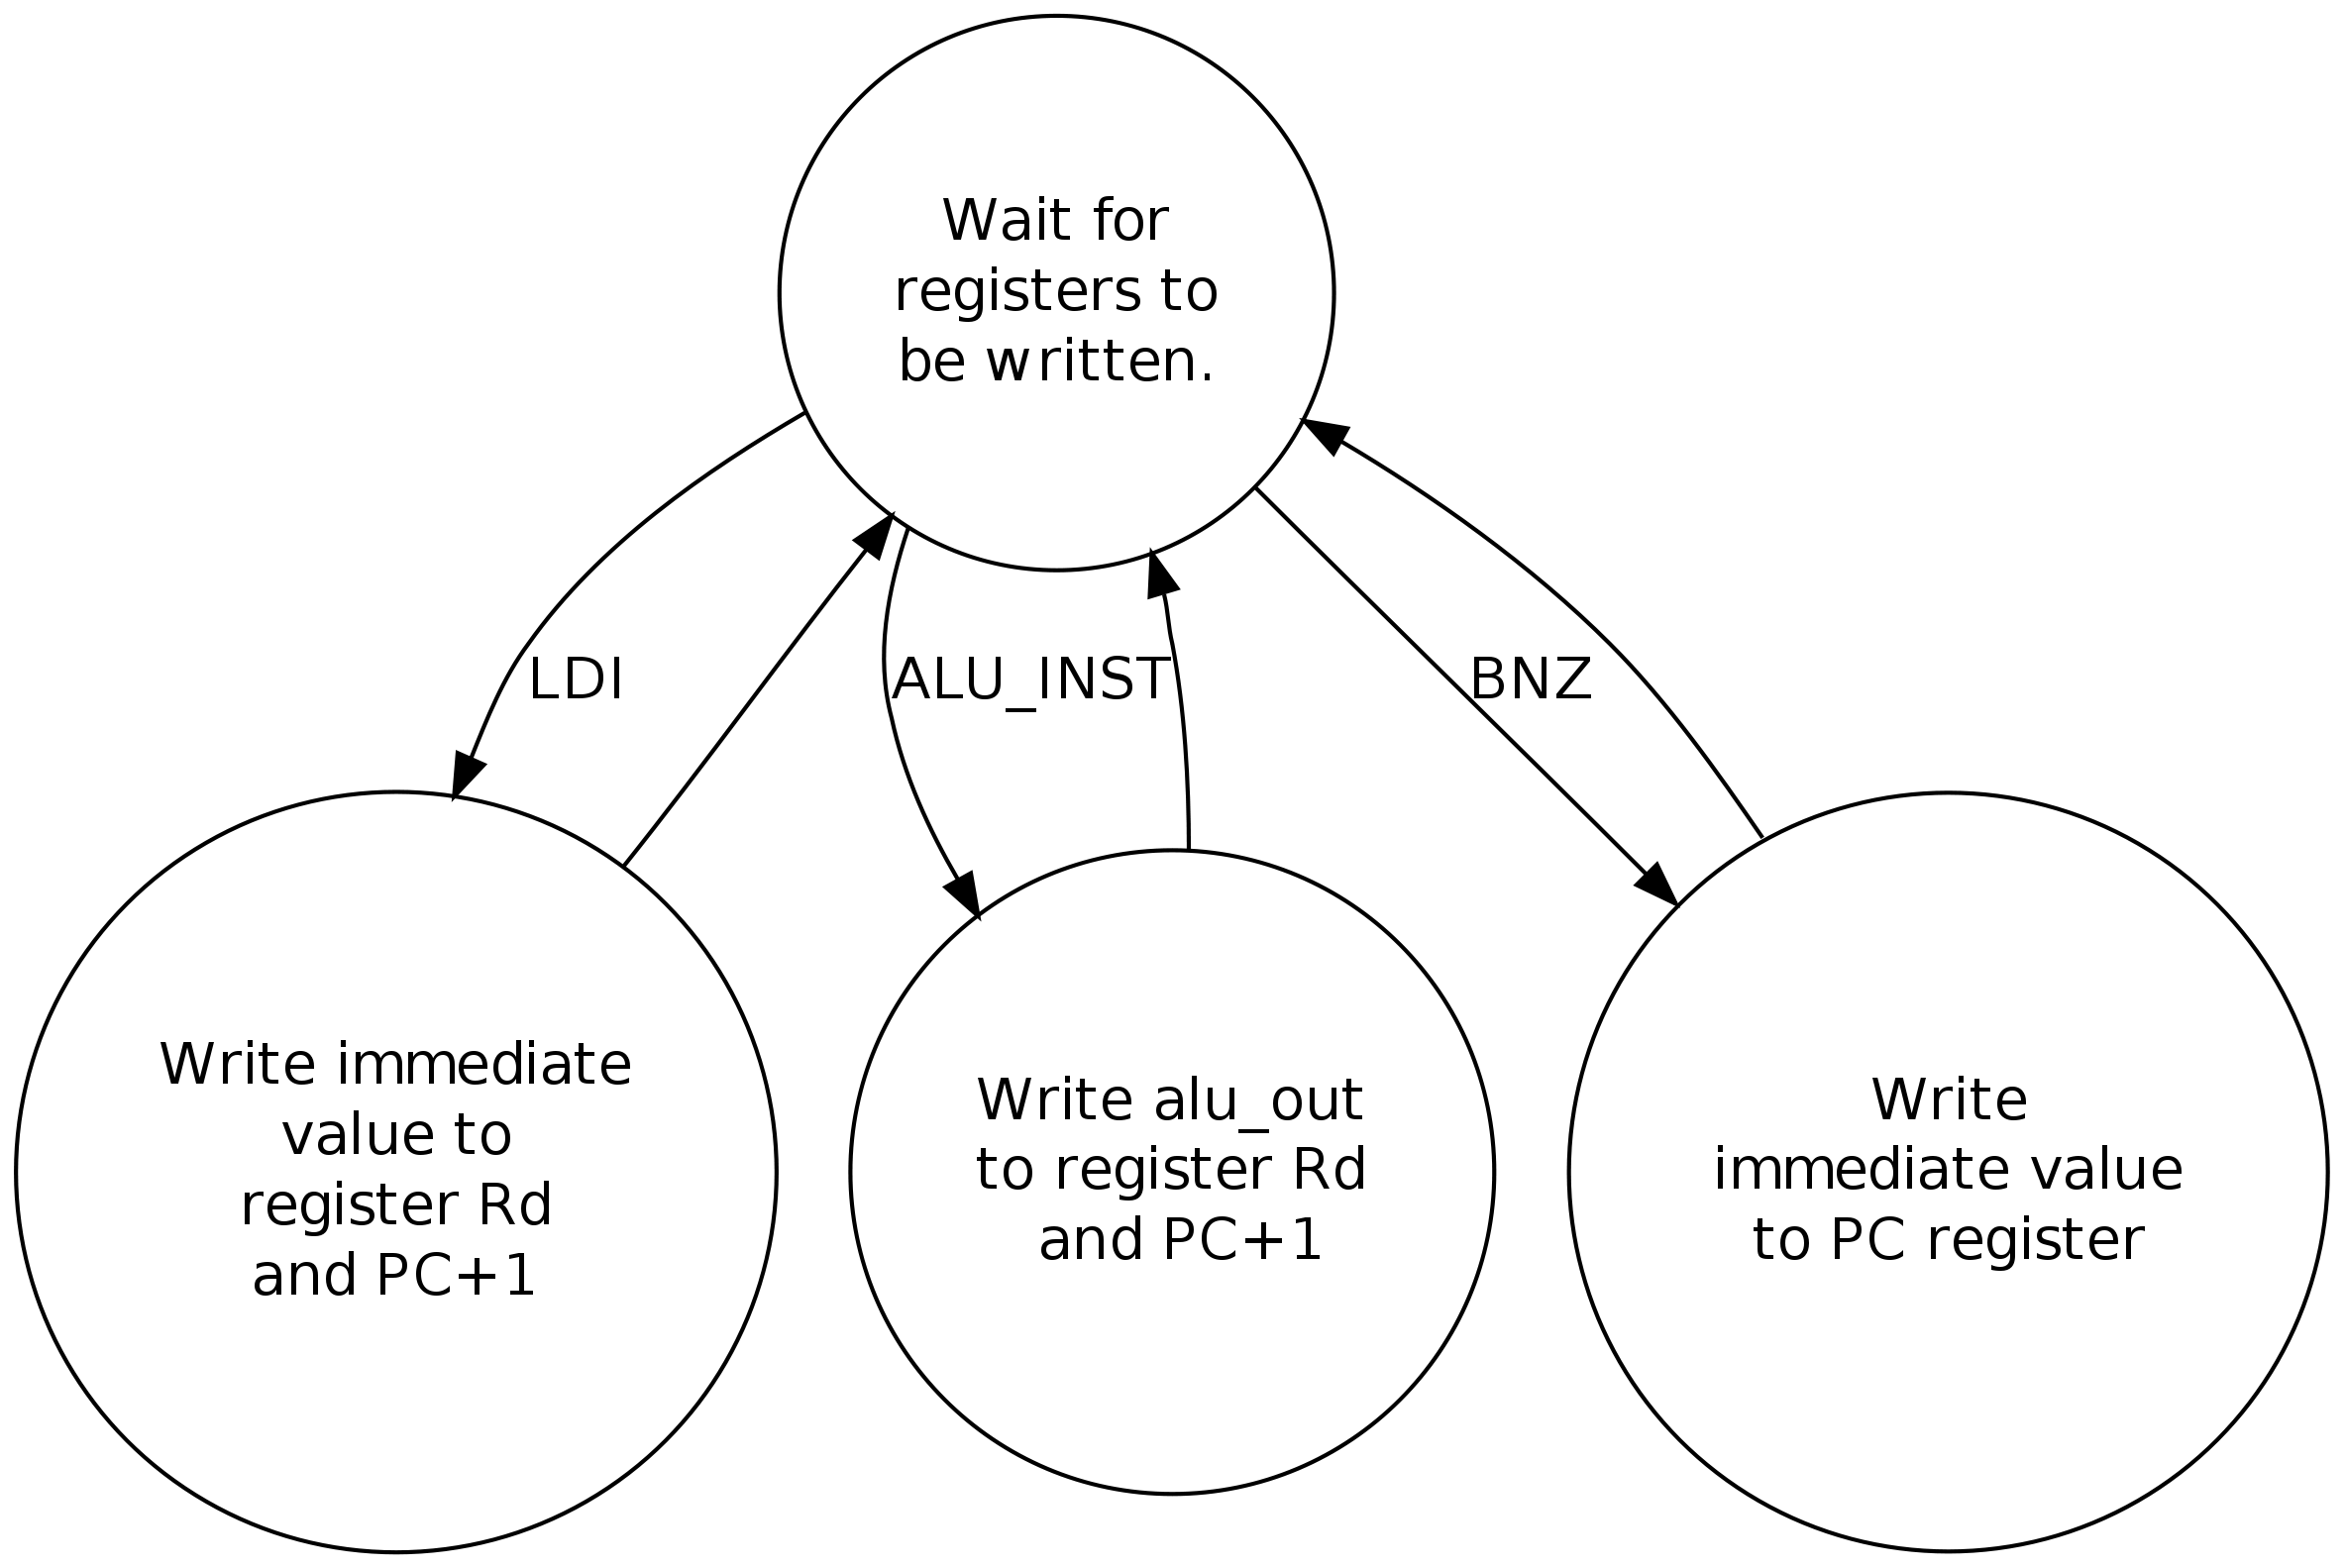
\includegraphics[width=.75\linewidth]{state_diagram.png} \\
  figure 1
\end{center}

\subsection*{Testing}

During the implementation process we wrote several testbenches
for the various components. We did not write any testbenches for the
components given to us, except the ALU. At the end, when all components were ready and
connected, we tested the entire design with a testbench for the cpu
component (cpu\_testbench.vhd).  We wrote this to be the main
testbench and implemented it using some procedures to create some
abstraction from the gory details.

\subsection*{Synthesis}

From the synthesis report we see that
\begin{enumerate}
\item The regfile muxer inferred 8 1-bit multiplexers, this was a
  little strange as we expected 1 8-bit multiplexer.  This does not
  matter to the functionality though.
\item The sr module inferred one D-type flip flop, this is exatly what
  we wanted.
\item The pc module inferred one 8-bit counter, this is also exactly
  what we wanted.
\item The control module inferred 1 D-type flip flop, this is used to
  hold the current state (fetch or execute), the rest is
  combinatorial, so this is also what we wanted.
\item the toplevel and cpu modules did not infer anything, which was
  expected as they are simply mapping signals between the other
  modules.
\end{enumerate}

\section*{Result}

% Present the result of the work. What works and what does not. 
% What the problems were if there were
% any. Or even better: what was fantastic in the group's work.
% Here is the place to add some screen-shots, debug outputs or similar to
% support the documentation. It is also the place to praise or show more
% critique towards the presented work.

Everything worked perfectly after a couple of days work, 
both simulation and testing on nalle. This was earlier than expected, 
but was probably due to increased knowledge and understanding of  
vhdl from the previous assignment, and the fact that we cooperated on it.


\section*{Evaluation}

% If there is something about the exercise what should be changed, 
% mention it here – text in the
% compendium, support files, exercise itself or something else which
% us as teaching staff should see to.

\section*{Conclusion}

% Round up - what works, what does not work. Comment on the exercise. 
% Write a bit about what was easy and what not so.

It was easy to map everything together and create most of the components. 
The most difficult part of this assignment was to figure out the timing 
and syncronization, when to write to the registers and when they where 
ready to be read.

\end{document}


